\documentclass[12pt]{article}
\usepackage[english]{babel}
\usepackage[utf8]{inputenc}
\usepackage{amsmath, amssymb, amsthm}
\usepackage{graphicx}
\usepackage{hyperref}
\usepackage[margin=.75in]{geometry}
\usepackage{xcolor}
\usepackage{tikz}

\newcommand{\id}{\text{id}}
\newcommand{\od}{\text{od}}

\setlength{\topmargin}{0pt}
\setlength{\headsep}{0pt}
\textheight = 600pt

\title{Graph Theory \\ Homework 16}
\author{Ben Kallus and Josef Komissar}
\date{Due Monday, April 26}

\begin{document}
\maketitle

\medskip\noindent\textbf{I (a)}

    We have previously shown that $Q_n$ is bipartite for all $n \in \mathbb N$.
    Thus, by K\"onig's Theorem, $\chi'(Q_n) = \Delta(Q_n) = n$.

\medskip\noindent\textbf{I (b)}

    The maximum vertex degree in the Gr\"otzsch graph is 5, so by Vizing's Theorem, the chromatic index of the Gr\"otzsch graph is either 5 or 6.
    The following drawing shows that the chromatic index of the Gr\"otzsch graph is 5.
    \begin{center} 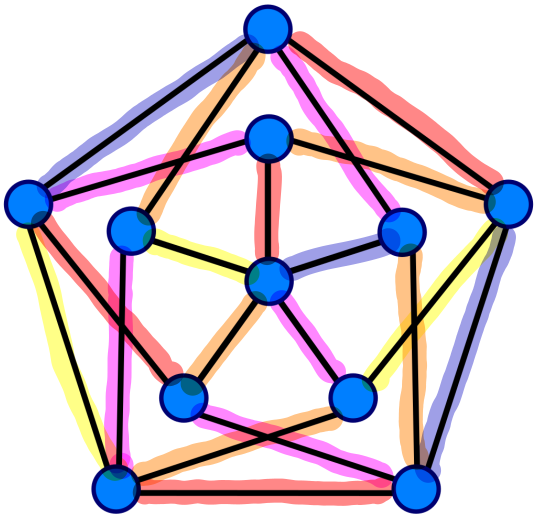
\includegraphics[scale=.5]{fig1.png} \end{center}

\medskip\noindent\textbf{I (c)}

    By Theorem 8.13, PG is not 1-factorable.
    Because PG is regular, by the special case we discussed in class following Theorem 10.13, $\chi'(PG) \neq 3$, so $\chi'(PG) = 4$.

\medskip\noindent\textbf{10.18} Proposition: If $H$ is a $2k$-regular graph of order $4k+1$ for some positive integer $k$, and $G$ is a subgraph of $H$ obtained by removing a set of $k-1$ independent edges from $H$, then $\chi'(G) = \Delta(G) + 1$.
\begin{proof}
    Let $k \in \mathbb Z^+$, and let $H$ be a $2k$-regular graph of order $n = 4k+1$.
    Let $G$ be a subgraph of $H$ obtained by removing a set of $k-1$ independent edges from $H$.
    Then, by the Handshaking Lemma, $|E(G)| = \frac{2k(4k+1)}{2} - (k-1) = 4k^2 + 1$.
    Thus,
    \begin{align*}
        |E(G)| &= 4k^2 + 1 \\
        &> 4k^2 \\
        &= \frac12 \cdot 2k \cdot 4k \\
        &= \frac12 \Delta(H) (n - 1) \\
        &\geq \frac12\Delta(G)(n-1).
    \end{align*}

    Thus, by Theorem 10.13, $\chi'(G) = 1 + \Delta(G)$.
\end{proof}

\medskip\noindent\textbf{II (a)} Proposition: If $G$ is a graph in which every vertex except one has degree $d \geq 1$, and $\chi'(G) = d$, then $G$ has odd order.
\begin{proof}
    Let $G$ be a graph in which every vertex except one has degree $d \geq 1$.
    Let $u$ be the vertex in $G$ that does not have degree $d$.
    Suppose that $\chi'(G) = d$.
    Suppose that $\deg(u) > d$.
    Then, each edge incident to $u$ must have a distinct color.
    Thus, $\chi'(G) > d$, which contradicts our assumption.
    Thus, $\deg(u) < d$.
    Because $\deg(u) < \chi'(G)$, there exists a color $c$ in a $d$-coloring of $G$ such that no $c$-colored edge is incident to $u$.
    Consider the set of all $c$-colored edges in $G$.
    Because all vertices in $G - u$ have degree $d$, and $\chi'(G) = d$, each of these vertices must be incident to exactly one $c$-colored edge.
    Thus, because the $c$-colored edges are independent, they constitute a perfect matching on $G-u$.
    Thus, $G-u$ has even order, so $G$ has odd order.
\end{proof}

\medskip\noindent\textbf{II (b)} Proposition: If $G$ is a graph in which every vertex except one has degree $d \geq 1$, and $\chi'(G) = d$, then $G$ has an isolated vertex.
\begin{proof}
    Let $G$ be a graph in which every vertex except one has degree $d \geq 1$.
    Let $u$ be the vertex in $G$ that does not have degree $d$.
    Suppose that $\chi'(G) = d$.
    Suppose that $\deg(u) > 0$.
    Then, there exists a color $c$ in a $d$-coloring of $G$ such that an edge of color $c$ is incident to $u$.
    Note that because $\chi'(G) = d$, and $\deg(v) = d$ for all $v \in V(G) \setminus \{u\}$, there exists a $c$-colored edge incident to each of these vertices.
    Thus, the set of all $c$-colored edges in $G$ induces a perfect matching in $G$.
    However, $G$ is of odd order, so it cannot have a perfect matching.
    Thus, $\deg(u) = 0$.
\end{proof}

\medskip\noindent\textbf{III} Proposition: If $G$ is a connected $d$-regular graph and $u$ is a cut-vertex of $G$, then $\chi'(G) = d+1$.
\begin{proof}
    Let $d \geq 1$, and let $G$ be a connected $d$-regular graph with cut-vertex $u$.
    Let $H$ be a component of $G-u$.
    Then, every edge that runs between a vertex in $H$ and a vertex in $G-H$ must be incident to $u$.
    Note that because $u$ is a cut-vertex, $u$ must be adjacent to at least one vertex $v$ in $G-H$.
    Thus, $G-H$ is connected, because the only vertex in $G-H$ that was affected by $H$'s removal is $u$, and $u$ is adjacent to $v$ in $G-H$.
    Then, every vertex in $G-H$ has degree $d$ except $u$.

    Suppose that $\chi'(G-H) = d$.
    Then, by \textbf{II (b)}, $G - H$ has an isolated vertex.
    This contradicts its connectedness, so $\chi'(G-H) = d+1$.
    Thus, $\chi'(G) \geq d+1$.
    Thus, by Vizing's Theorem, $\chi'(G) = d + 1$.
\end{proof}

\medskip\noindent\textbf{IV} Proposition: If $G$ is planar of order $n < 12$, then $\chi(G) \leq 4$.
\begin{proof}
    Note that for any planar graph $G$ of order $n \leq 4$, $\chi(G) \leq 4$ since each vertex can be colored a different color.
    Let $G$ be a planar graph of order $n \leq 11$ and assume there is a four-coloring of every planar graph of order $n-1$.
    By Theorem 9.15, $\delta(G) \leq 4$.
    Let $v\in V(G)$ be a vertex such that $\deg v \leq 4$.
    We can color $G-v$ with the four colors blue, green, red, and orange by the inductive hypothesis.
    If $v$'s neighbors have less than four distinct colors in the coloring for $G-v$, we will have a color available for $v$ to create a four-coloring for $G$.
    Otherwise, $\deg v = 4$ and each neighbor of $v$ has a different color.
    Given a planar embedding of $G$, label the neighborhood of $v$ as follows:
    \begin{center} 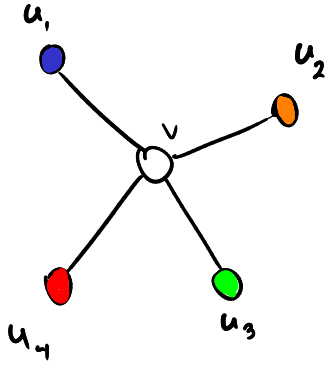
\includegraphics[scale=.4]{fig2.png} \end{center}
    
    Consider the subgraph $H_{gb}$ of $G$ induced by $G$'s green and blue vertices.
    If $u_1$ and $u_3$ are in different components of $H_{gb}$, then we can switch the colors in $u_1$'s component so no neighbor of $v$ is blue.
    Then, coloring $v$ blue gives a four-coloring of $G$.
    If $u_1$ and $u_3$ are in the same component of $H_{gb}$, then there is a green-blue $u_1-u_3$ path in $G$.
    Now, consider the subgraph $H_{ro}$ of $G$ induced by $G$'s red and orange vertices.
    If $u_2$ and $u_4$ are in different components of $H_{ry}$, then we can switch the colors in $u_2$'s component so no neighbor of $v$ is red.
    Then, coloring $v$ red gives a four-coloring of $G$.
    Otherwise, there must be a red-orange $u_2-u_4$ path in $G$, which must cross the green-blue $u_1-u_3$ path, contradicting the planarity of $G$.
    Thus, $G$ has a four-coloring, so $\chi(G) \leq 4$.
\end{proof}

\medskip\noindent\textbf{V (a)}
To free up red, we would have to flip the colors of the red-green and red-yellow components containing the two red regions next to the uncolored region. However, flipping the colors in these components would turn the uppermost green area to red and the lower yellow area to red, putting two red areas adjacent to one another and making it an invalid coloring. Thus, red cannot be freed up.

\pagebreak
\medskip\noindent\textbf{V (b)}
\begin{center} 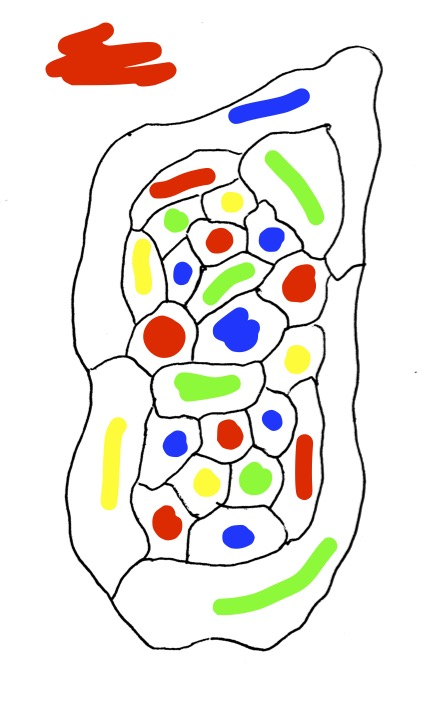
\includegraphics[scale=.5]{heawood.jpg} \end{center}

\end{document}
